\documentclass[conference]{IEEEtran}
\IEEEoverridecommandlockouts
\usepackage{amsmath,amssymb,amsfonts}
\usepackage{algorithmic}
\usepackage{graphicx}
\usepackage{textcomp}
\usepackage{xcolor}
\def\BibTeX{{\rm B\kern-.05em{\sc i\kern-.025em b}\kern-.08em
    T\kern-.1667em\lower.7ex\hbox{E}\kern-.125emX}}
\begin{document}

\title{Performance Metrics for Evaluating Internet Speed Test in Symmetric Broadband\\
}

\author{\IEEEauthorblockN{1\textsuperscript{rd} Nathan Joshua Sucgang}
\IEEEauthorblockA{\textit{Department of Electronics, Computer, and Communications Engineering} \\
\textit{Ateneo De Manila University}\\
Quezon City, Philippines \\
nathan.sucgang@student.ateneo.edu}
\and
\IEEEauthorblockN{2\textsuperscript{rd} Geoffrey Miguel Guy}
\IEEEauthorblockA{\textit{Department of Electronics, Computer, and Communications Engineering} \\
\textit{Ateneo De Manila University}\\
Quezon City, Philippines \\
geoffrey.guy@student.ateneo.edu}
}

\maketitle

\begin{abstract}
    The internet has become more than a routine of everyone's life; 
    it has become a necessity. This paper aims to use statistics to identify the different factors that affect many aspects of the internet such as its download speed, upload speed, and ping. 
    The research looks at various factors for the causes and changes in the internet's performance such as the location of the household receiving the signal for their internet. 
    With this research information, the researchers of the paper intend to determine which possible factors hamper the internet's performance metrics in order to leave the issue in the hands of organizations who have the capacity to combat these same hindrances. 
    This data could also further improve the internet performance for the population, consequently improving a conventional part of urban societal life.
\end{abstract}

\begin{IEEEkeywords}
ping, download speed, upload speed, internet
\end{IEEEkeywords}

\section{Random Variables and Sources of Data}
\begin{enumerate}
    \item[1.]
    \textbf{Location}:
    The location of the closest test server when the test was being conducted.

    \textbf{Source}: Data gathered from the Ookla Speedtest using Raspberry Pi 4. 
    \item[2.]    
    \textbf{Download Speed}: 
    How fast you can receive data from the internet to your device (measured in Mbps).

    \textbf{Source}: Data gathered from the Ookla Speedtest using Raspberry Pi 4. 
    \item[3.]
    \textbf{Upload Speed}:
    How fast you can send data from your device to the internet (measured in Mbps). 
    
    \textbf{Source}: Data gathered from the Ookla Speedtest using Raspberry Pi 4. 
    \item[4.]
    \textbf{Ping}: 
    A type of latency measurement that sends a small packet of data from your device to a server and back (measured in ms).

    \textbf{Source}: Data gathered from the Ookla Speedtest using Raspberry Pi 4. 
    \item[5.] 
    \textbf{Jitter}: 
    Variation in latency over time (measured in ms).

    \textbf{Source}: Data gathered from the Ookla Speedtest using Raspberry Pi 4. 
    \item[6.] 
    \textbf{Latency}: 
    Time it takes for data to travel from your device to a server and back (measured in ms).

    \textbf{Source}: Data gathered from the Ookla Speedtest using Raspberry Pi 4. 
\end{enumerate}

\section{Normality of Data}
\begin{enumerate}
    \item[1.]    
    \textbf{Download Speed}: 
    \begin{enumerate}
        \item \textbf{Test}: Kolmogorov-Smirnov Test
        \item \textbf{Result}: D = 1, p-value $<$ 2.2e-16 (not normal)
    \end{enumerate}

    \item[2.]
    \textbf{Upload Speed}:
    \begin{enumerate}
        \item \textbf{Test}: Kolmogorov-Smirnov Test
        \item \textbf{Result}: D = 1, p-value $<$ 2.2e-16 (not normal)
    \end{enumerate}

    \item[3.]
    \textbf{Ping}:
    \begin{enumerate}
        \item \textbf{Test}: Kolmogorov-Smirnov Test
        \item \textbf{Result}: D = 0.81376, p-value $<$ 2.2e-16 (not normal)
    \end{enumerate}

    \item[4.] 
    \textbf{Download Jitter}: 
    \begin{enumerate}
        \item \textbf{Test}: Kolmogorov-Smirnov Test
        \item \textbf{Result}: D = 0.60492, p-value $<$ 2.2e-16 (not normal)
    \end{enumerate}

    \item[5.] 
    \textbf{Upload Jitter}: 
    \begin{enumerate}
        \item \textbf{Test}: Kolmogorov-Smirnov Test
        \item \textbf{Result}: D = 0.78504, p-value $<$ 2.2e-16 (not normal)
    \end{enumerate}

    \item[6.] 
    \textbf{Ping Jitter}: 
    \begin{enumerate}
        \item \textbf{Test}: Kolmogorov-Smirnov Test
        \item \textbf{Result}: D = 0.50309, p-value $<$ 2.2e-16 (not normal)
    \end{enumerate}

    \item[7.]   
    \textbf{Download Average Latency}: 
    \begin{enumerate}
        \item \textbf{Test}: Kolmogorov-Smirnov Test
        \item \textbf{Result}: D = 0.87014, p-value $<$ 2.2e-16 (not normal)
    \end{enumerate}

    \item[8.]   
    \textbf{Upload Average Latency}: 
    \begin{enumerate}
        \item \textbf{Test}: Kolmogorov-Smirnov Test
        \item \textbf{Result}: D = 0.88351, p-value $<$ 2.2e-16 (not normal)
    \end{enumerate}
\end{enumerate}

\section{Methodology}
\begin{figure}[htbp]
\centerline{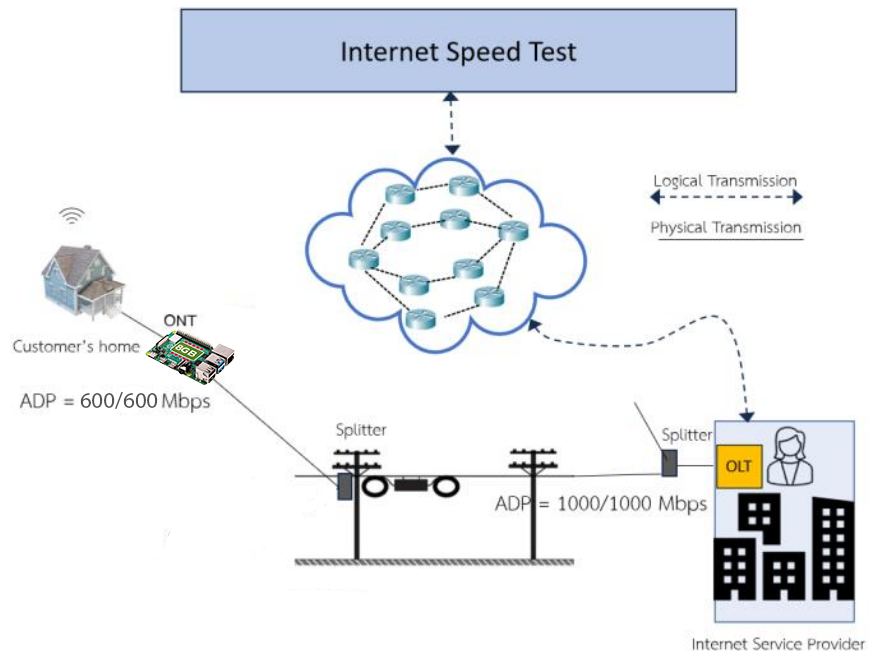
\includegraphics[width=8cm,height=6cm,keepaspectratio]{experimental_setup.png}}
\caption{A scenario in evaluating internet speed test.}
\label{fig1}
\end{figure}
As shown in Fig. 1. The Methodology involve collecting data from the Ookla Speedtest using Raspberry Pi 4.
The experiment was conducted from June 18 to June 30, 2024 amounting to 1116 data points. The dataset was cleaned by removing any test from Globe Telecom, any error that came with misconfigured network.
Statistical analyses, including box plot, map graph, regression analysis, time series graph, was used to examined the relationship between download speed, upload speed, ping, jitter, and latency.
MS Excel and R was used to analyze the data. The statistical analysis was done to determine the factors that affect the internet speed test.

\begin{thebibliography}{00}
\bibitem{b1} A. Boonsongsrikul et al., "Performance Metrics and Strategy for Evaluating Internet Speed Tests in Fixed Broadband Networks," 2024 IEEE International Conference on Big Data and Smart Computing (BigComp), Bangkok, Thailand, 2024, pp. 424-428, doi: 10.1109/BigComp60711.2024.00093.
\bibitem{b2} A. Saengsai et al., "Broadband Internet Speed Dashboard for Sustainable Service Improvement in Thailand," 2024 IEEE International Conference on Big Data and Smart Computing (BigComp), Bangkok, Thailand, 2024, pp. 418-423, doi: 10.1109/BigComp60711.2024.00092. 
\bibitem{b3} C. Overturf., “How does Speedtest measure my network speeds?” SPEEDTEST. https://help.speedtest.net/hc/en-us/articles/360038679354-How-does-Speedtest-measure-my-network-speeds (accessed June 30, 2024)
\bibitem{b4} E. M. Rio, Jr.,  “rules and regulations implementing republic act (r.a.) no. 10929 known as the free internet access in public places act”, DICT. https://dict.gov.ph/wp-content/uploads/2017/12/IRR-RA-10929-Version-8.pdf (accessed June 30, 2024).
\bibitem{b5} G. S. Ford, “Comparative Analysis of Fixed Broadband Speeds in Cities Across the World”, ResearchGate, Jan, 2022, doi: 10.2139/ssrn.4159788
\bibitem{b6} R. B. Ikhsan, G. Mohammed, I. Putriana, T. Sriwidadi, Aries and J. W. Wahono, "Customer Loyalty Based On Internet Service Providers-Service Quality," 2022 6th International Conference on Informatics and Computational Sciences (ICICoS), Semarang, Indonesia, 2022, pp. 18-23, doi: 10.1109/ICICoS56336.2022.9930615.
\bibitem{b7} R. Sharma, M. Richardson, G. Martins, and N. Feamster, “Measuring the Prevalence of WiFi Bottlenecks in Home Access Networks,” arXiv, Nov. 9 2023, doi: 10.48550/arxiv.2311.05499.
\bibitem{b8} S. Bebortta and S. K. Das, "Assessing the Impact of Network Performance on Popular E-Learning Applications," 2020 Sixth International Conference on e-Learning (econf), Sakheer, Bahrain, 2020, pp. 61-65, doi: 10.1109/econf51404.2020.9385497.
\bibitem{b8} W. Woo and S. Hasan, “What's my Daily Value? Interpretation of network performance metrics in broadband consumer labels”, Association for Computing Machinery, New York, NY, USA, 2023, pp. 8-24, doi: 10.1145/3609396.3610546
\bibitem{b9} X. Deng, Y. Fung, T. Sutjarittham, H. H. Gharakheili, B. Gallego, V. Sivaraman, “Comparing Broadband ISP Performance using Big Data from M-Lab”, arXiv, Jan. 24, 2021, doi: 10.48550/arXiv.2101.09795.
\end{thebibliography}

\end{document}
